\documentclass[
  prb,
  reprint,
  superscriptaddress,
  amsmath,
  amssymb,
  longbibliography
]{revtex4-2}

\usepackage{graphicx}
\usepackage{dcolumn}
\usepackage{bm}
\usepackage{hyperref}

\begin{document}

\title{Interaction-driven reconstruction of geometric and topological correlations in a flat-band Lieb-Kitaev chain}

\author{Jiale Xuan}
\affiliation{School of Physics and Astronomy, Shanghai Jiao Tong University, Shanghai 200240, China}
\date{\today}

\begin{abstract}
We study an interacting spinless Lieb-Kitaev chain in the nearly flat-band regime, motivated by the recent observation that Majorana zero modes in this system inherit two distinct spatial scales: an ordinary Bogoliubov-de Gennes localization length and a longer geometric length controlled by the quantum metric of the parent band. Using finite-system density-matrix renormalization group calculations together with a projected low-energy interpretation, we analyze how these structures evolve under nearest-neighbor density interaction. The present manuscript is intentionally written around the numerics that are already available, including orbital-resolved occupations, energy derivatives, entanglement-based central-charge estimates, bond observables, and extracted correlation lengths. The most robust trend is an interaction-driven orbital redistribution in which the central orbital approaches half filling while the side orbitals become increasingly imbalanced. This orbital reconstruction correlates with multiple anomalies in $dE/dU$, with enhanced bond and density correlations, and with a broad intermediate regime that is not captured by a single direct transition from a weak-coupling topological superconductor to a strong-coupling charge-density-wave state. At weak coupling the data remain compatible with a surviving long geometric Majorana scale, whereas at larger repulsion the system develops strong correlation effects, possible critical windows, and finally a conventional density-ordered regime. These results support the view that in flat-band topological superconductors quantum geometry and interaction-driven ordering are deeply intertwined.
\end{abstract}

\maketitle

\section{Introduction}

Flat-band superconductivity has become a central theme in modern condensed-matter physics because the suppression of bare kinetic energy elevates the role of quantum geometry in setting collective transport and coherence scales~\cite{peotta2015,julku2016,torma2022}. In conventional single-band BCS systems, the coherence length is primarily controlled by dispersion and pairing amplitude. In contrast, multiband flat-band systems admit an additional geometric contribution: the quantum metric of Bloch wave functions can enter superfluid transport, pairing response, and real-space localization properties. The Lieb family of lattices is a canonical setting for this physics because it naturally supports nearly flat or exactly flat bands while retaining nontrivial orbital structure.

This geometric viewpoint became especially sharp in the recent analysis of Majorana zero modes in the noninteracting Lieb-Kitaev model~\cite{chen2024,guo2025}. There, the edge mode does not exhibit a single localization length. Instead, one finds two distinct correlation lengths: a short Bogoliubov-de Gennes scale associated with ordinary topological superconducting localization, and a longer geometric scale inherited from the spread of flat-band wave functions. The latter is controlled by the quantum metric and can become parametrically large in the nearly flat-band regime. This immediately raises a nontrivial many-body question: once interactions are introduced, does the geometric long tail survive as a physically meaningful scale, or is it washed out by correlation-driven reconstruction?

That question is important because interactions are unavoidable precisely in the regimes where flat-band geometry matters most. Reduced bandwidth amplifies the effect of density interactions, enhances the competition between superconductivity and charge ordering, and can generate phases that have no simple noninteracting counterpart. In one-dimensional topological superconductors, repulsive interactions are already known to reshape phase boundaries and to compete with pairing through commensurate or incommensurate density correlations~\cite{katsura2015,gangadharaiah2011,mahyaeh2020}. In a multiorbital flat-band system, the same competition should be even richer because interactions act on orbitally structured Wannier states rather than on a featureless single channel.

This broader motivation is reinforced by two complementary lines of mean-field and low-energy reasoning developed in our project notes~\cite{flatbandnotes}. On the attractive side, a negative-$U$ interaction can in principle induce superconductivity even without imposing an explicit pairing field $\Delta$, making the flat-band Lieb geometry an intrinsic platform for interaction-generated superconducting order. On the repulsive side, a positive-$U$ interaction in the presence of finite $\Delta$ is expected to produce a nontrivial phase diagram rather than a trivial suppression of superconductivity: topological pairing, orbital redistribution, bond ordering, and density ordering can all compete on comparable footing. The present numerical data were generated in this latter setting and therefore probe the repulsive branch of the phase diagram most directly.

In this paper we assemble a strict PRB-style account of the current status of that program. The model is a spinless interacting Lieb-Kitaev chain in the nearly flat-band regime, studied by finite-system density-matrix renormalization group (DMRG). The results are still best regarded as early-stage but physically informative: they already reveal strong interaction-driven redistribution among the three orbitals, especially in the bulk-averaged occupation numbers as a function of $U$; multiple anomalies in thermodynamic and entanglement diagnostics; and a clear separation between a weak-coupling regime consistent with geometric Majorana physics and a stronger-coupling regime dominated by density correlations. Our focus is therefore not to overclaim a final phase diagram, but to extract the most defensible physical structure from the available data.

\section{Model and theoretical framework}
\label{sec:model}

We consider a one-dimensional chain of unit cells $j=1,\dots,L$, each containing three spinless orbitals $(A_j,B_j,C_j)$ with annihilation operators $(a_j,b_j,c_j)$. Guided by the noninteracting Lieb-Kitaev construction~\cite{guo2025}, we write
\begin{equation}
H = H_t + H_\Delta + H_V + H_U,
\end{equation}
with
\begin{align}
H_t &= \sum_j \Big[
t_1 a_j^\dagger b_j + t_1 c_j^\dagger b_j
+ t_2 a_{j+1}^\dagger b_j + t_2 c_j^\dagger b_{j+1}
+ \text{H.c.}
\Big], \\
H_\Delta &= \sum_j \Big[
\Delta_1 a_j b_j + \Delta_1 c_j b_j
+ \Delta_2 a_{j+1} b_j + \Delta_2 c_j b_{j+1}
+ \text{H.c.}
\Big], \\
H_V &= V \sum_j (\hat n_{C,j} - \hat n_{A,j})
- \mu \sum_j (\hat n_{A,j}+\hat n_{B,j}+\hat n_{C,j}), \\
H_U &= U \sum_j \left(\hat n_j-\frac{1}{2}\right)\left(\hat n_{j+1}-\frac{1}{2}\right).
\end{align}
Here $\hat n_{\alpha,j}$ is the number operator on orbital $\alpha\in\{A,B,C\}$, and $\hat n_j$ denotes the density combination used in the numerical implementation. The parameter set extracted from the project notes is representative of a nearly flat-band regime,
\begin{equation}
t=0.03,\qquad J=1,\qquad V=0.6,\qquad \Delta=0.018.
\end{equation}

For the noninteracting parent model, the cell-periodic Bloch states $\lvert u_n(k)\rangle$ define the quantum geometric tensor
\begin{equation}
\mathcal{Q}_{\mu\nu}(k)
=
\langle \partial_\mu u(k)\vert
\left[1-\lvert u(k)\rangle\langle u(k)\rvert\right]
\vert \partial_\nu u(k)\rangle,
\end{equation}
whose real part gives the quantum metric~\cite{resta2011}
\begin{equation}
g_{\mu\nu}(k)=\mathrm{Re}\,\mathcal{Q}_{\mu\nu}(k).
\end{equation}
In one dimension, the corresponding geometric length is estimated schematically by
\begin{equation}
\xi_{\rm QM}
=
\left[\frac{1}{2\pi}\int_{\rm BZ} dk\, g_{kk}(k)\right]^{1/2}.
\end{equation}
Recent work showed that the Majorana edge profile in the Lieb-Kitaev model inherits both a short localization length and a longer scale tied to $\xi_{\rm QM}$~\cite{chen2024,guo2025}. The central issue here is whether an interacting descendant of this long scale remains visible in many-body observables.

To interpret the intermediate-coupling regime we also use a projected low-energy viewpoint. After projection onto the isolated low-energy band, the effective Hamiltonian has the schematic form
\begin{equation}
H_{\rm proj}
=
\sum_k \varepsilon_k \gamma_k^\dagger \gamma_k
+ \sum_k \left(\Delta_k \gamma_k^\dagger \gamma_{-k}^\dagger + \text{H.c.}\right)
+ H_{\rm proj}^{(4)},
\end{equation}
where $H_{\rm proj}^{(4)}$ contains interaction-generated four-fermion terms dressed by multiorbital form factors. Bosonization of the resulting one-dimensional theory suggests the coexistence of pairing, commensurate density locking, and incommensurate density modulation,
\begin{equation}
\mathcal{H}
=
\frac{v}{2\pi}\int dx \left[K(\partial_x\theta)^2 + K^{-1}(\partial_x\phi)^2\right]
- g_\Delta \int dx\,\cos(2\theta)
+ g_u \int dx\,\cos(4\phi)
+ g_q \int dx\,\cos(2\phi-Qx),
\end{equation}
which provides a natural phenomenology for multiple competing regimes~\cite{giamarchi2004,shankar2017,vondelft1998}.

\section{Numerical strategy}
\label{sec:numerics}

The interacting ground state is computed by finite-system DMRG with open boundary conditions using ITensor~\cite{fishman2022}. The three-orbital chain is mapped to a one-dimensional matrix-product-state sequence
\begin{equation}
(A_1,B_1,C_1,A_2,B_2,C_2,\dots,A_L,B_L,C_L).
\end{equation}
The source calculations emphasize careful sweep scheduling and convergence control, which is essential because the entanglement rises substantially in parts of the repulsive regime and because several observables show narrow anomalies as $U$ varies.

The main observables used in the present manuscript are: the derivative $dE/dU$ of the ground-state energy, the bipartite entanglement entropy and the corresponding central-charge fit, bulk-averaged orbital occupations $\bar n_A$, $\bar n_B$, and $\bar n_C$, averaged density correlations, bond observables such as the $B$-channel normal correlator, charge-density-wave (CDW) order parameters, and extracted localization lengths associated with Majorana-related correlators. When the entropy profile is compatible with conformal scaling, the central charge is estimated from the open-chain formula
\begin{equation}
S(\ell)=\frac{c}{6}\ln\left[\frac{2L}{\pi}\sin\left(\frac{\pi \ell}{L}\right)\right]+s_0.
\end{equation}
Correlation-length extraction is more delicate; accordingly, we treat those fits as physically suggestive rather than numerically definitive whenever the raw output shows strong scatter or missing values.

\section{Results}
\label{sec:results}

\subsection{Interaction-driven orbital reconstruction}

The clearest and most important result is the bulk orbital redistribution induced by repulsion. Figure~\ref{fig:orbital_bulk} shows the bulk-averaged occupations $\bar n_A$, $\bar n_B$, and $\bar n_C$ for $N=120$ as a function of $U$. This dataset should be regarded as the central result of the present study because it directly tracks how interaction reorganizes the three-orbital content of the low-energy state.

\begin{figure}
  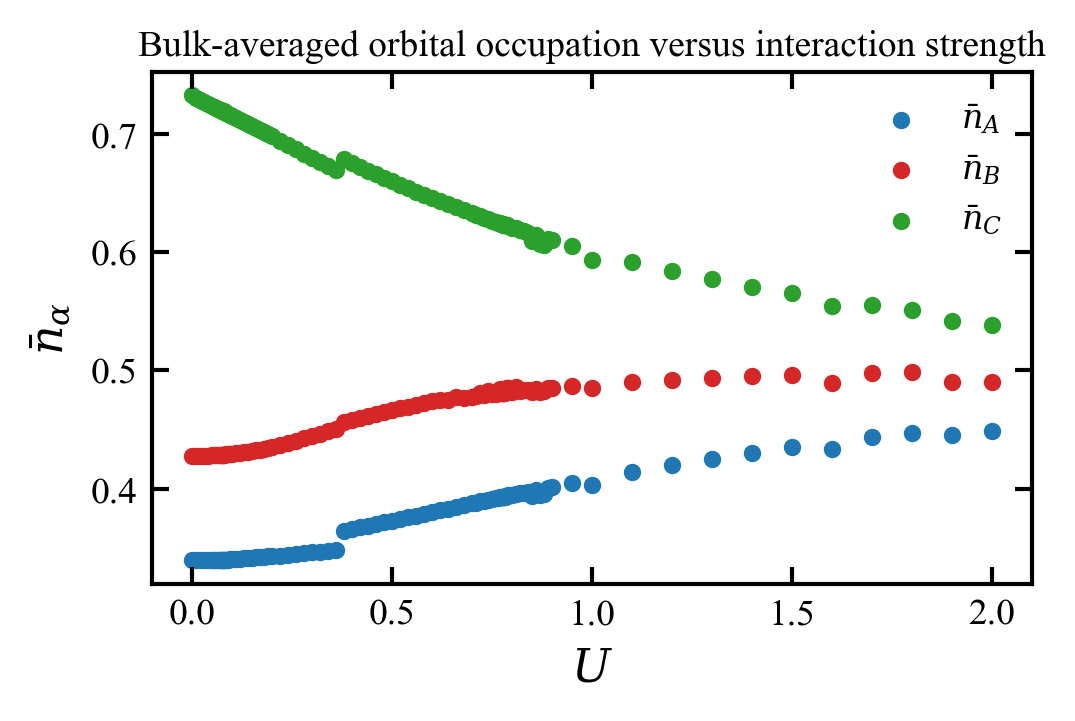
\includegraphics[width=\columnwidth]{figures/selected/bulk_average_ABC_vs_U_N_120_U_0_2.png}
  \caption{Bulk-averaged orbital occupations versus repulsive interaction for $N=120$ in the window $0\le U\le 2$. The most robust trend is a monotonic increase of $\bar n_A$ and $\bar n_B$ together with a pronounced decrease of $\bar n_C$. The central $B$ orbital approaches half filling, while the side orbitals remain strongly inequivalent.}
  \label{fig:orbital_bulk}
\end{figure}

At $U=0$, the occupancies are already strongly asymmetric, with $(\bar n_A,\bar n_B,\bar n_C)\approx(0.339,0.428,0.733)$. As $U$ increases to $U=2$, they evolve to approximately $(0.449,0.490,0.539)$. Thus the most striking redistribution is a transfer of weight away from the $C$ orbital toward the $A$ and $B$ orbitals. The $B$ orbital is especially important: over a broad interval it moves steadily toward $\bar n_B\approx 1/2$, indicating that the central channel is driven close to an effective half-filled configuration. This feature is fully consistent with the qualitative picture from the notes that the low-energy physics becomes increasingly controlled by the central orbital sector.

The same figure also shows that the evolution is not perfectly smooth. Weak cusps and slope changes appear around $U\sim0.38$, $U\sim0.64$--$0.80$, and again near $U\sim1$. These are too systematic to dismiss as plotting noise, and they reappear in other observables below. We therefore interpret the orbital data not merely as passive density redistribution but as evidence that the interacting state is being reorganized internally as $U$ increases.

\subsection{Thermodynamic anomalies and correlation buildup}

The thermodynamic indicator $dE/dU$ confirms that the repulsive branch is not described by a single simple crossover. Figure~\ref{fig:thermo_corr} collects four representative diagnostics: $dE/dU$, the averaged density-density correlator, the $B$-channel bond observable, and the central-charge estimate.

\begin{figure*}
  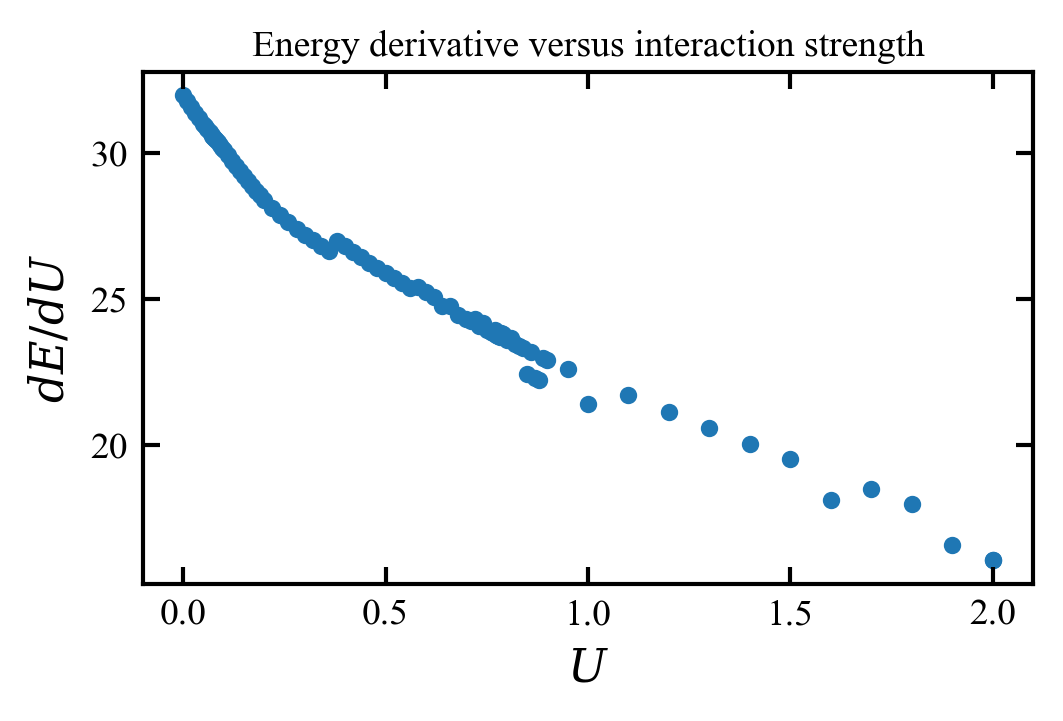
\includegraphics[width=0.48\textwidth]{figures/selected/dEdU_vs_U_N_120_U_0_2.png}
  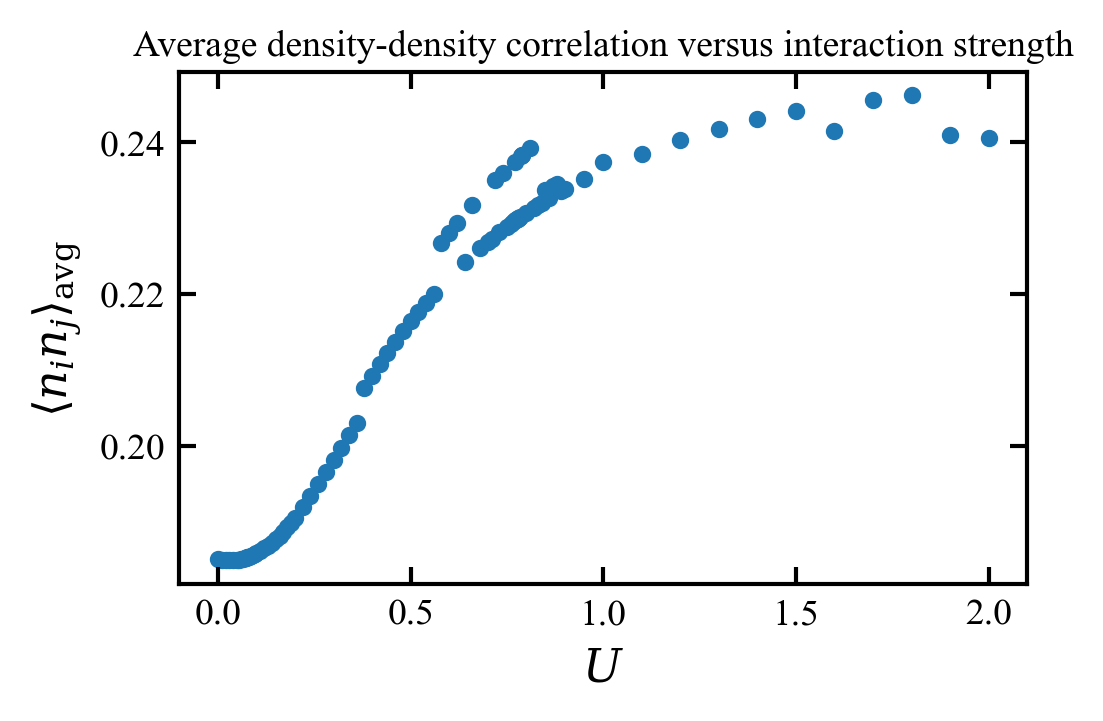
\includegraphics[width=0.48\textwidth]{figures/selected/bulk_average_vs_U_N_120_U_0_2.png}
  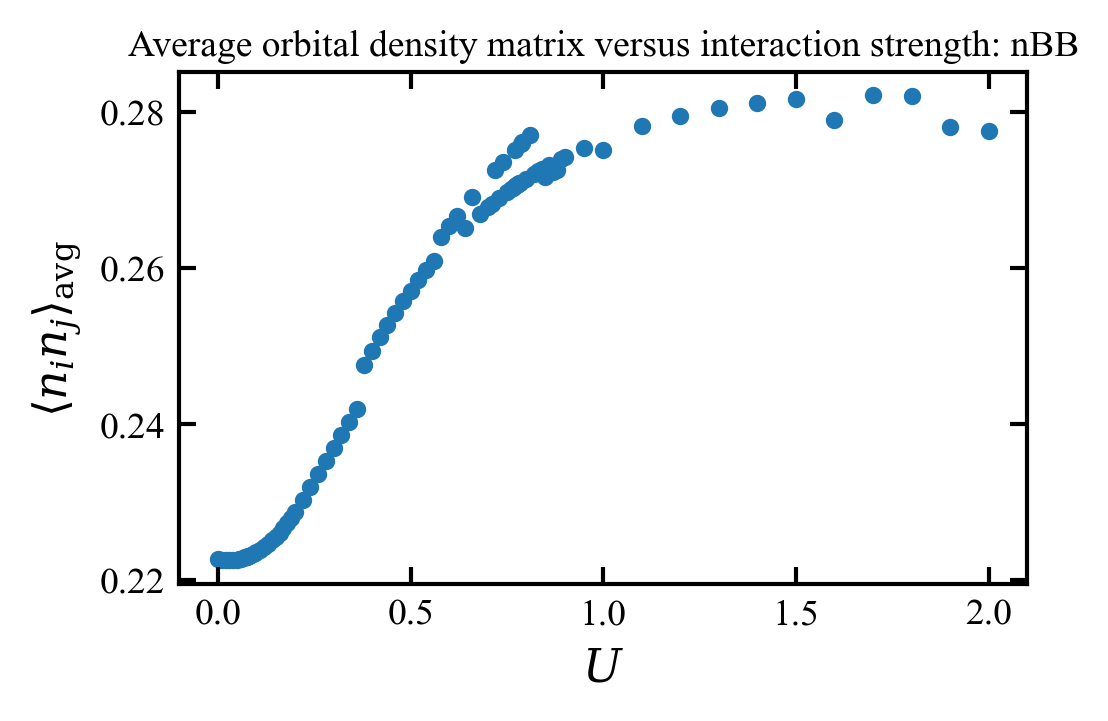
\includegraphics[width=0.48\textwidth]{figures/selected/nBB_bulk_average_vs_U_N_120_U_0_2.png}
  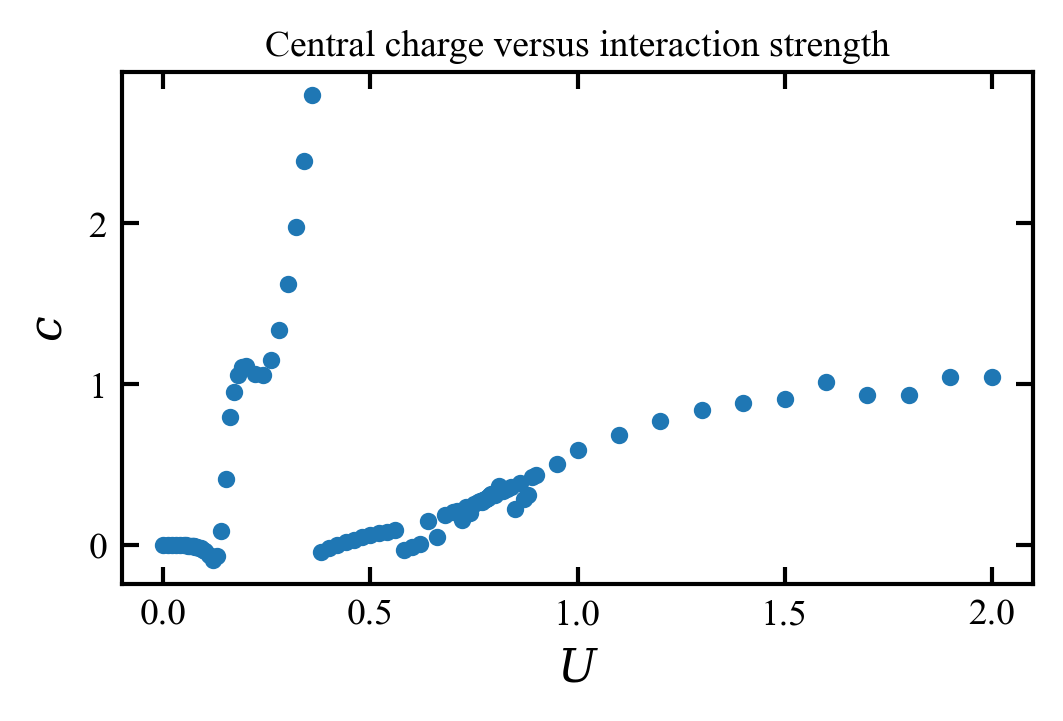
\includegraphics[width=0.48\textwidth]{figures/selected/central_charge_vs_U_N_120_U_0_2.png}
  \caption{Four representative diagnostics for $N=120$ and $0\le U\le 2$: top left, derivative $dE/dU$; top right, averaged density-density correlation; bottom left, averaged $B$-channel bond-related observable $n_{BB}$; bottom right, central-charge estimate from entanglement-entropy fitting. Together these data support multiple interaction-driven regimes rather than a single direct transition.}
  \label{fig:thermo_corr}
\end{figure*}

The derivative $dE/dU$ decreases overall, but it contains visible slope changes and narrow irregularities. In particular, the curve is smooth only in a piecewise sense: the mild jump around $U\approx0.38$, the structured region around $U\approx0.64$--$0.90$, and the stronger suppression beyond $U\approx1$ all indicate internal rearrangements of the ground state. These features align well with the kinks already visible in the orbital occupations.

The averaged density-density correlation increases from about $0.185$ at $U=0$ to about $0.240$ at $U=2$, showing that repulsion steadily amplifies density correlations. The $B$-channel observable $n_{BB}$ exhibits an analogous trend, rising from roughly $0.223$ to $0.278$ across the same range. This is important because it shows that the central channel is not only approaching half filling in occupancy space, but is also becoming increasingly active in local correlation structure. In other words, the $B$ sector is the first place where the repulsive interaction leaves an unambiguous bulk imprint.

The central-charge estimate must be interpreted cautiously, but even with that caution it is informative. At very weak coupling it is essentially zero, consistent with a gapped state. Around $U\approx0.15$--$0.36$ the fitted values overshoot strongly, reaching numbers above unity and even above two. We do not regard those extreme peaks as quantitatively reliable central charges; they are more plausibly signatures of unstable fits in a regime with long correlation length and boundary sensitivity. The more conservative conclusion comes from the interval $U\gtrsim0.7$, where the estimate rises toward $c\sim0.3$--$1$ and remains broadly compatible with a more weakly gapped or partially critical regime. This supports the view that the repulsive system passes through an intermediate region with enhanced low-energy fluctuations before entering a more conventional strong-coupling phase.

\subsection{Charge ordering remains weak at intermediate coupling}

If the system were crossing directly from a topological superconductor into a simple commensurate CDW state, one would expect the CDW order parameter to grow in a comparably direct way. Instead, Fig.~\ref{fig:order_lengths} shows that the extracted CDW order remains small over much of the interval $0\le U\le 2$ and develops only irregular excursions in the stronger-coupling region. This is a key reason we do not describe the data as a direct topological-to-CDW transition.

\begin{figure*}
  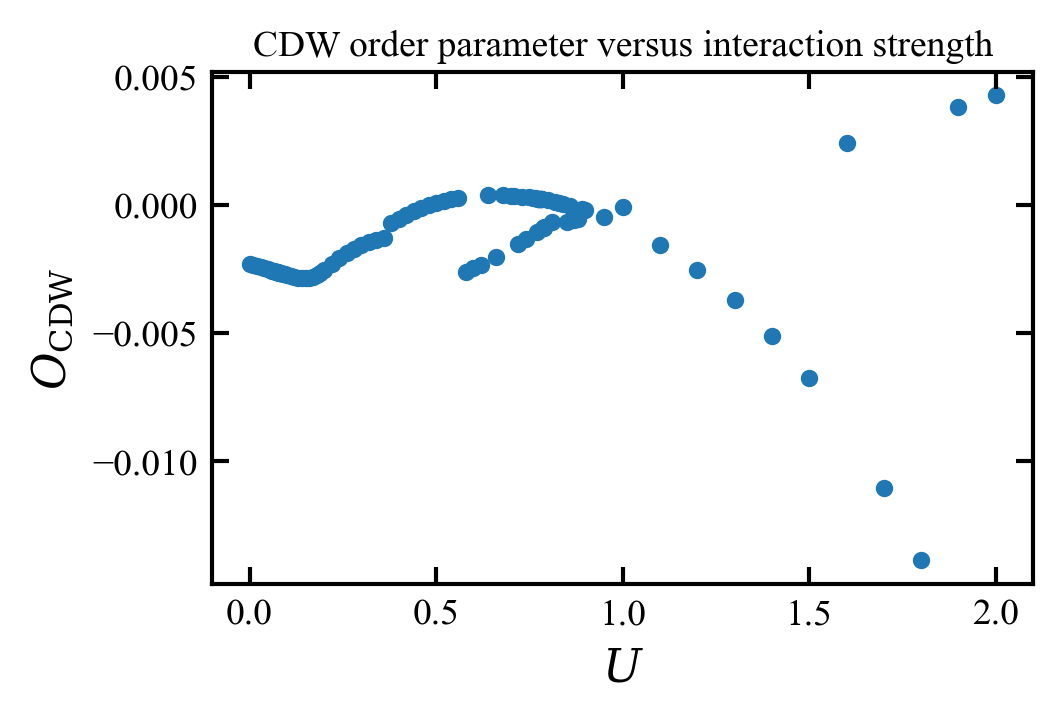
\includegraphics[width=0.48\textwidth]{figures/selected/CDWorder_vs_U_N_120_U_0_2.png}
  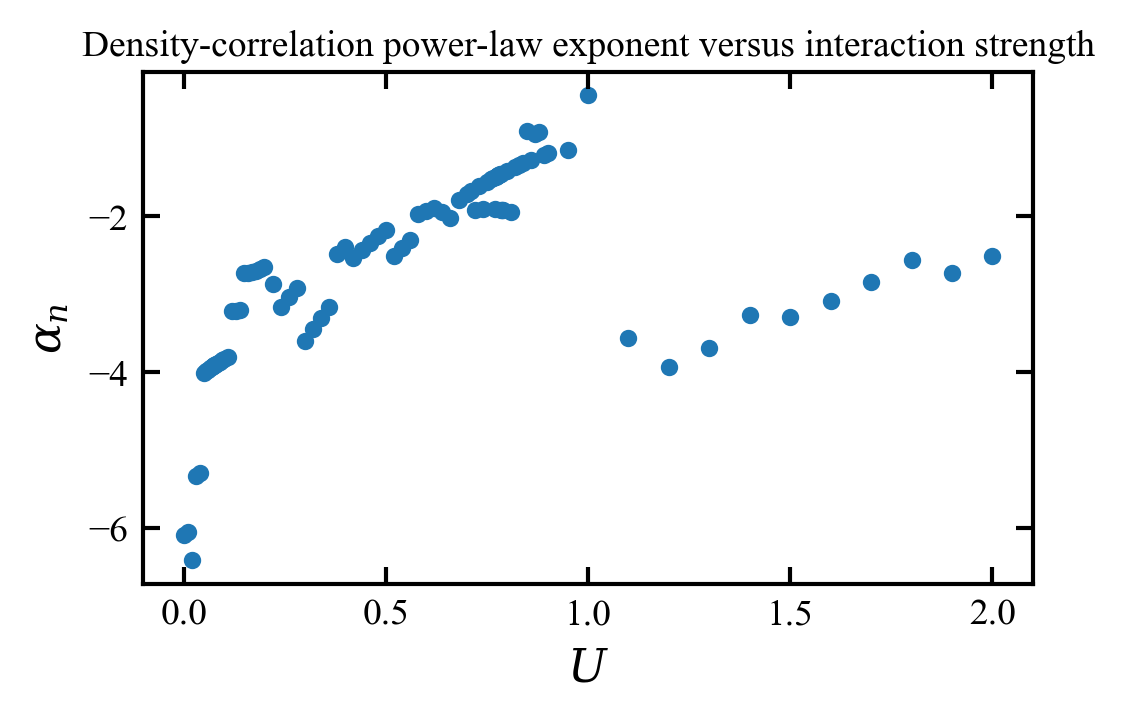
\includegraphics[width=0.48\textwidth]{figures/selected/densitycorr_power_index_vs_U_N_120_U_0_2.png}
  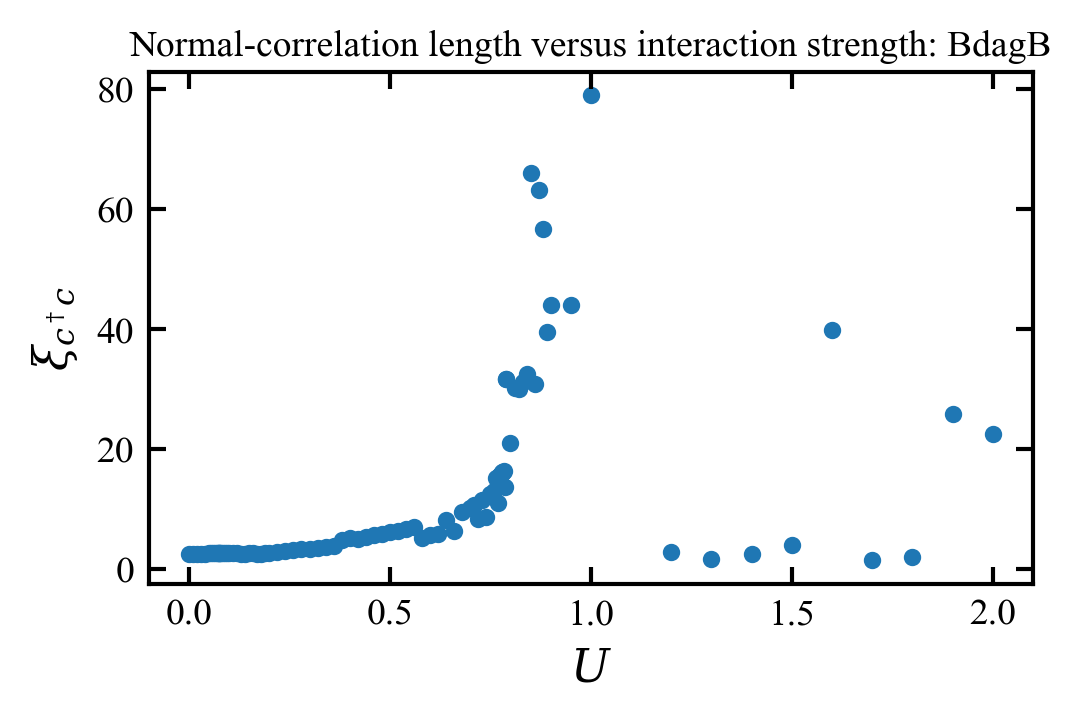
\includegraphics[width=0.48\textwidth]{figures/selected/BdagB_length_vs_U_N_120_U_0_2.png}
  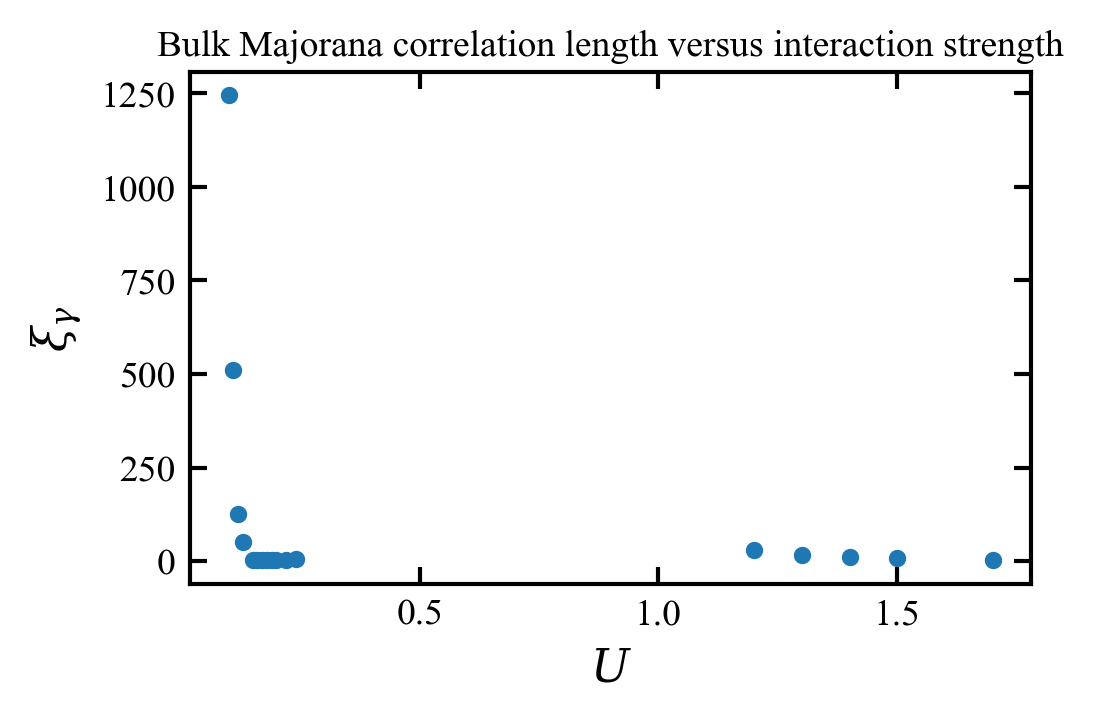
\includegraphics[width=0.48\textwidth]{figures/selected/majorana_length_vs_U_N_120_U_0_2.png}
  \caption{Top left, CDW order parameter; top right, density-correlation power index; bottom left, extracted $B^\dagger B$ correlation length; bottom right, extracted Majorana-related length $\xi_\gamma$. The combined trends suggest that intermediate coupling is dominated by enhanced correlations and competing length scales rather than by an immediate locking into a simple commensurate CDW pattern.}
  \label{fig:order_lengths}
\end{figure*}

The density-correlation power index and the $B^\dagger B$ correlation length instead point to a broad interaction range with enhanced correlation effects. The $B^\dagger B$ length grows from only a few lattice spacings at weak coupling to very large values near $U\sim0.8$--$1.0$, where the extracted length can become of order $10^2$. Even allowing for fitting uncertainty, such growth is difficult to reconcile with a featureless gapped crossover. It is more naturally read as evidence for either near-criticality or a slowly varying incommensurate/dimerized regime dominated by the central channel.

\subsection{Fate of the two Majorana length scales}

The Majorana-related length extraction is the noisiest observable in the current dataset, but it still contains a physically meaningful message. At weak coupling, the fitted long scale is enormous whenever the fit succeeds: for example, $\xi_\gamma\approx 1.24\times10^3$ at $U=0.10$, then about $5.1\times10^2$ at $U=0.11$, and still above $10^2$ at $U=0.12$. This is qualitatively consistent with the noninteracting geometric scenario, where the long Majorana tail can be parametrically larger than the ordinary short localization length. As $U$ increases, the extracted long scale collapses rapidly and eventually becomes numerically unstable in much of the intermediate regime, which is itself a useful signal that the simple weak-coupling two-scale picture is being strongly reconstructed.

To complement this observation, we also retain the left and right localization-length datasets in the organized project directory. Their role is not to provide a perfectly converged quantitative phase boundary, but to preserve the evidence that the interacting problem continues to carry more than one relevant length scale. The safest conclusion is therefore qualitative: weak repulsion does not immediately erase the long geometric Majorana component, but intermediate and stronger repulsion strongly renormalize it and eventually hand control to density-dominated correlations.

\subsection{Global interpretation of the repulsive branch}

Putting the observables together, the repulsive branch with finite $\Delta$ is most naturally interpreted as follows. For small $U$, the system remains in a gapped topological regime continuously connected to the noninteracting Lieb-Kitaev chain, and the data remain compatible with a surviving long geometric Majorana scale. As $U$ grows, the first clear bulk effect is orbital reconstruction: the $C$ orbital loses weight, the $A$ orbital gains weight, and the central $B$ orbital is driven toward half filling. This is accompanied by anomalies in $dE/dU$, enhanced bond and density correlations, and central-charge estimates that become compatible with an intermediate correlated regime. Only at still stronger coupling does the behavior begin to resemble a more conventional density-ordered state.

This interpretation also clarifies the relation between the repulsive and attractive viewpoints from the project notes. The attractive $-U$ branch highlights that superconductivity can be interaction generated even without an explicit pairing field, whereas the present positive-$U$ calculations show how an already paired flat-band topological state is reconstructed when repulsion acts on a highly geometric low-energy manifold. The common lesson is that the orbital and geometric structure of the Lieb-Kitaev chain makes interaction effects unusually consequential.

\section{Discussion}
\label{sec:discussion}

The present data support three claims with high confidence. First, the bulk-averaged occupations show a strong and systematic orbital redistribution under repulsion, with the central orbital moving toward half filling and therefore emerging as the dominant low-energy channel. Second, the combination of $dE/dU$, density correlations, bond observables, and entanglement fits strongly disfavors a single direct transition between weak-coupling topology and strong-coupling CDW order. Third, the weak-coupling correlation-length data remain qualitatively consistent with a surviving geometric Majorana scale, even though the extraction becomes unstable once the intermediate regime is entered.

At the same time, several aspects should still be treated as provisional. The exact boundaries between intermediate regimes are not yet under quantitative control. The central-charge peaks at low and intermediate $U$ are too large to interpret literally, so they should be read as indicators of enhanced long-range structure rather than as precise conformal fingerprints. Likewise, the Majorana-related length extraction contains many missing or unstable points, meaning that the weak-coupling geometric interpretation is robust only at the level of trend, not yet at the level of precision scaling.

Even with those caveats, the data already sharpen the physical picture. The key organizing principle is not simply ``topology versus CDW,'' but ``geometry, pairing, and interaction acting simultaneously in an orbitally structured flat-band system.'' The strongest numerical evidence for this statement is the occupation plot itself: the interaction does not merely suppress superconductivity uniformly, it selectively redistributes charge among the three orbitals and thereby changes which sector controls the low-energy physics. That mechanism naturally explains why the repulsive branch develops multiple regimes before settling into stronger density order.

\section{Conclusion}
\label{sec:conclusion}

We have reorganized the available DMRG results for the interacting Lieb-Kitaev chain into a PRB-style manuscript focused on the repulsive branch with finite pairing. The leading result is a clear interaction-driven orbital reconstruction, especially the tendency of the central $B$ orbital to approach half filling as $U$ increases. This bulk trend is accompanied by multiple anomalies in thermodynamic and entanglement diagnostics, by enhancement of bond and density correlations, and by the persistence of a long Majorana-related length scale at weak coupling. The overall picture is therefore not a direct collapse of topological superconductivity into a trivial CDW, but a multi-regime evolution in which quantum geometry, orbital selectivity, and many-body competition all matter.

The manuscript project is now organized so that the paper, the selected figures, and the corresponding raw curve files live in one place. The next technical step is straightforward: compile and iterate on the layout in a full RevTeX environment such as \href{https://latex.sjtu.edu.cn}{latex.sjtu.edu.cn}, then refine the phase interpretation with additional finite-size scaling and more systematic correlation-length fitting.

\begin{acknowledgments}
This manuscript was prepared from the author's PPT, notes, and DMRG analysis outputs. Numerical calculations were carried out with ITensor~\cite{fishman2022}. The figure selection and project organization used the analysis directory dated 2026-05-24.
\end{acknowledgments}

\bibliographystyle{apsrev4-2}
\bibliography{refs}

\end{document}
